\hypertarget{ux30bbux30afux30b7ux30e7ux30f3section}{%
\section{セクション(section)}\label{ux30bbux30afux30b7ux30e7ux30f3section}}

\hypertarget{ux30b5ux30d6ux30bbux30afux30b7ux30e7ux30f3subsection}{%
\subsection{サブセクション(subsection)}\label{ux30b5ux30d6ux30bbux30afux30b7ux30e7ux30f3subsection}}

\hypertarget{ux30b5ux30d6ux30b5ux30d6ux30bbux30afux30b7ux30e7ux30f3subsubsection}{%
\subsubsection{サブサブセクション(subsubsection)}\label{ux30b5ux30d6ux30b5ux30d6ux30bbux30afux30b7ux30e7ux30f3subsubsection}}

吾輩は猫である。名前はまだ無い。

どこで生れたかとんと見当がつかぬ。何でも薄暗いじめじめした所でニャーニャー泣いていた事だけは記憶している。吾輩はここで始めて人間というものを見た。しかもあとで聞くとそれは書生という人間中で一番|獰悪な種族であったそうだ。

\begin{multicols}{2}
この書生というのは時々我々を捕えて煮て食うという話である
\footnote{
寿限無、寿限無
五劫の擦り切れ
海砂利水魚の
水行末 雲来末 風来末
食う寝る処に住む処
藪ら柑子の藪柑子
パイポ パイポ パイポのシューリンガン
シューリンガンのグーリンダイ
グーリンダイのポンポコピーのポンポコナーの
長久命の長助
}
。しかしその当時は何という考もなかったから別段恐しいとも思わなかった。ただ彼の掌に載せられてスーと持ち上げられた時何だかフワフワした感じがあったばかりである。


\begin{itembox}[l]{公式}
$e^{i \pi} = -1$
\end{itembox}

\begin{description}
\item[項目] 説明
\item[Keyword]\mbox{}\\
    long description 長い説明
    long description 長い説明
    long description 長い説明
\end{description}

\begin{itemize}
    \item 箇条書き
    \begin{itemize}
        \item 第2レベル箇条書き
        \begin{itemize}
            \item 第3レベル箇条書き
            \begin{itemize}
                \item 第4レベル箇条書き
            \end{itemize}
        \end{itemize}
    \end{itemize}
\end{itemize}

\begin{table}[H]
\centering
\caption{sample table \label{tab:ta}}
\begin{tabular}{|c|c|} \hline
a & b \\ \hline
c & d \\ \hline
\end{tabular}
\end{table}

\begin{lstlisting}[language=python,caption=hello code \label{src:hello}]
while True:
    print("hello world")
\end{lstlisting}

\end{multicols}

\begin{figure}[H]
\begin{minipage}{0.5\hsize}
    \centering
    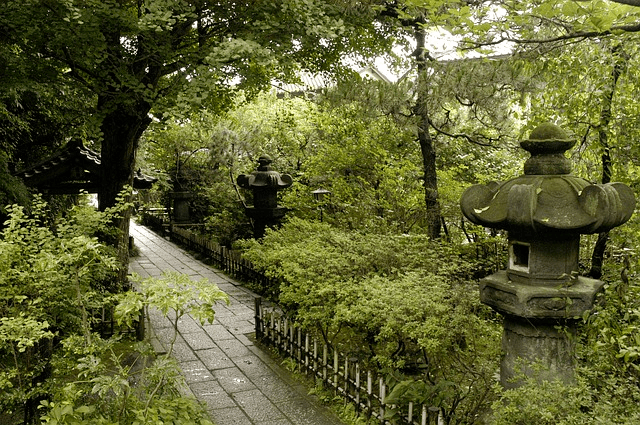
\includegraphics[width=6cm]{./sample/1.png}
    \subcaption{left \label{fig:2fig1}}
\end{minipage}
\begin{minipage}{0.5\hsize}
    \centering
    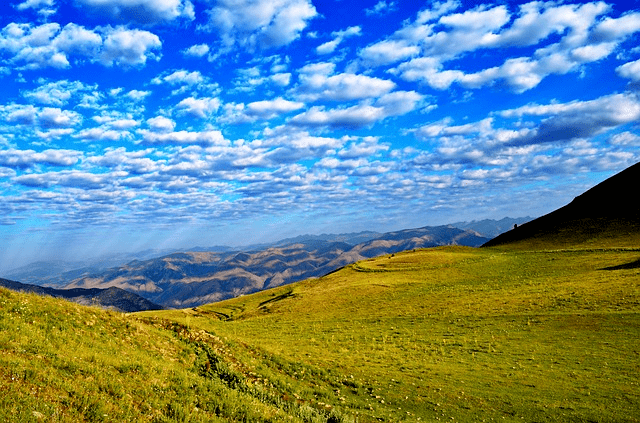
\includegraphics[width=6cm]{./sample/2.png}
    \subcaption{right \label{fig:2fig2}}
\end{minipage}
\caption{2 figures \label{fig:2fig}}
\end{figure}
